% Forrás: Fleiner Tamás gyakorlat

\documentclass[tikz]{standalone}
\usepackage{tikz}
\usetikzlibrary{positioning, graphs}
\usetikzlibrary{graphs.standard}
\begin{document}
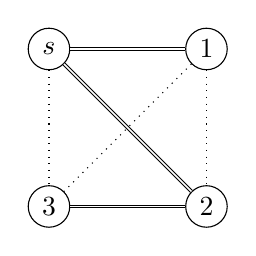
\begin{tikzpicture}
		[vertex/.style={draw,circle,inner sep = 0mm, minimum size = 15},
         edgelabel/.style = {fill = white, inner sep = 2, font=\small}]

        \node[vertex] (a) at (0, 0) {$s$};
        \node[vertex] (b) at (2, 0) {$1$};
        \node[vertex] (c) at (2, -2) {$2$};
        \node[vertex] (d) at (0, -2) {$3$};

        \draw[double] (a) to (b);
        \draw[double] (a) to (c);
        \draw[dotted] (a) to (d);
        \draw[dotted] (b) to (c);
        \draw[dotted] (b) to (d);
        \draw[double] (c) to (d);
		
\end{tikzpicture}
\end{document}